\item \begin{theorem}{()} \quad\quad
    \begin{itemize}
        \item For any uniform cost RAM program $T(n) = \Omega(S(n))$, where $S(n)$ is the space an algorithm uses for an input of size $n$.
        \item The capacity of each edge of a flow network can be floating-point, and it can be solved by linear programming.
        \item (100NYCU-57c) The value of any flow of a flow network is bounded by the capacity of only at most $O(2^n)$ cuts.
        \item (109NYCU-2) 2-coloring: $O(n^2)$, 3-coloring, 4-coloring: superpolynomial.
        \item Weighted-union heuristic: Append the \textbf{smaller} list onto the \textbf{longer} list, with ties broken arbitrarily.
        \item $n! \neq \Theta(n^n)$.
        \item A DAG with $n$ vertices can \textbf{NOT} have more than $\binom{n}{2}$ edges.
        \item Longest palindrome subsequence: \begin{equation}
            \begin{aligned}
                & L(i, j) = \begin{cases}
                    0 &, i = j + 1 \\
                    1 &, i = j \\
                    L(i + 1, j - 1) + 2 &, i < j \land s[i] = s[j] \\
                    \max(L(i + 1, j), L(j, j - 1)) &, \text{otherwise}
                \end{cases} \\
                & \text{where} \ L[1 \cdots n][1 \cdots n], s[1 \cdots n]
            \end{aligned}
        \end{equation}
        \item (102NTU-4) Minimum triangulation: \begin{equation}
            c(i, j) = \begin{cases}
                0 &, j < i + 2 \\
                \min\limits_{i < k < j}\{c(i, k) + c(k, j) + dist(i, j) + dis(j, k) + dist(k, j)\} &, \text{otherwise}
            \end{cases}
        \end{equation} \begin{lstlisting}[caption={Minimum triangulation.}, captionpos=b]
            double triangulation(Point P[], int n) {
                if (n < 3)
                    return 0;
                
                double c[n][n];
                for (int gap = 0, gap < n; gap++) {
                    for(int i = 0, j = gap; j < n; i++, j++) {
                        if (j < i + 2)
                            c[i][j] = 0.0;
                        else {
                            c[i][j] = MAX;
                            for (int k = i + 1; k < j; k++) {
                                double val = c[i][k] + c[k][j] + wt(P, i, j, k);
                                if (c[i][j] > val)
                                    c[i][j] = val;
                            }
                        }
                    }
                }

                return c[0][n - 1];
            }
        \end{lstlisting}
        \item Sort $n$ integers ranged from $0$ to $n^2 - 1$: 將$n$個整數表示成\textbf{n進位}數,每個數由$2$-digit表示,範圍$0$到$n - 1$,再用radix sort對$2$-digit排序,共兩次。
        \item If max frequency is $\le 2$ times of min frequency, Huffman code is \textbf{NOT} always better than an ordinary fixed-length code.
        \item Amortized analysis與average-case analysis無關。
        \item (104NYCU-28b) (\textbf{FALSE}) \textbf{If} a graph has a unique MST then, for every cut of the graph, there is a \textbf{unique light edge} crossing the cut.
        \item (104NYCU-28c) (\textbf{TRUE}) A graph has a unique MST \textbf{if}, for every cut of the graph, there is a \textbf{unique light edge} crossing the cut.
        \item The worst-case running time and expected running time are equal to within \textbf{constant} factors for any randomized algorithm.
        \item Selection problem: $T(n) = T(\frac{n}{5}) + T(\frac{3n}{4}) + O(n)$
        \item Given an \textbf{undirected} graph and a positive integer $k$, is there a path of length $\le k$, which each edge has weight $1$ and each vertex is visited \textbf{exactly} once: P, solved by Floyd-Warshall algorithm.
        \item Given an \textbf{undirected} graph and a positive integer $k$, is there a path of length $\ge k$, which each edge has weight $1$ and each vertex is visited $\le$ once: NPC.
        \item A flow network of multiple sources can be reduced to a single source.
        \item Subset sum: \\
        $s(i, j)$: sum $j$ can be found in $\{a_1, \ \cdots, a_i\}$ \begin{equation}
            s(i, j) = \begin{cases}
                0 &, i = 0 \\
                1 &, j = 0 \\
                s(i - 1, j) \lor s(i - 1, j - v_i) &, j \ge v_i
            \end{cases}
        \end{equation} result is \begin{equation}
            s(m, n)
        \end{equation}
        \item Hanoi tower:
        \begin{itemize}
            \item Iterative version: Check if the \textbf{input number} $n$ is even or odd. \\ 
                If $n$ is even, \begin{equation}
                    \begin{cases}
                        A \leftrightarrow C \\
                        A \leftrightarrow B \\
                        C \leftrightarrow B
                    \end{cases} 
                \end{equation} If $n$ is odd, \begin{equation}
                    \begin{cases}
                        A \leftrightarrow B \\
                        A \leftrightarrow C \\
                        B \leftrightarrow C
                    \end{cases} 
                \end{equation}
            \item Convert to undirected graph and solved by Hamiltonian path problem: 
                \begin{figure}[H]
                    \centering
                    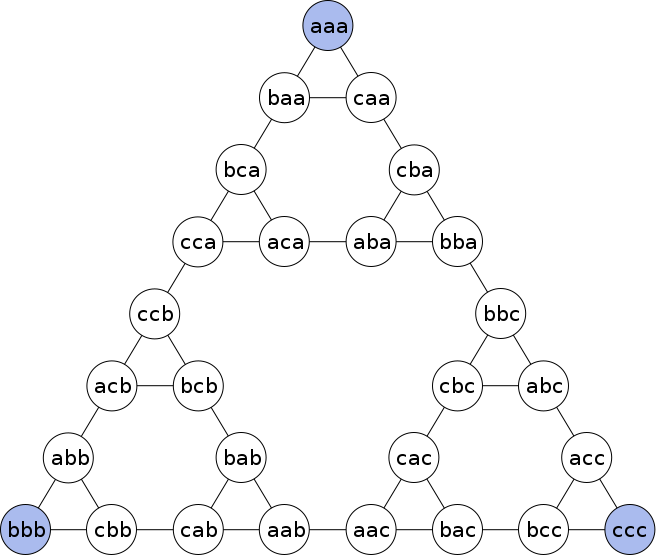
\includegraphics[scale=0.3]{img/hanoi_tower_graph.png}
                    \caption{Example of Hanoi tower converted to undirected graph and solved by Hamiltonian path problem. For each node, disk positions from left to right in order of increasing size, and edges represent moves.}
                    \label{img:hanoi-tower-graph}
                \end{figure}
        \end{itemize}
        \item Fibonacci search: \begin{lstlisting}[caption={Fibonacci search.}, captionpos=b, language=Python]
            def fibSearch(arr, data):
                max = len(arr) - 1
                y = getY(fib, max + 1) # Find the largest index, which its value is smaller than data.
                m = max - fib[y] 
                x = y - 1
                i = x
                if arr[i] < data: # Check at first.
                    i += m
                while fib[x] > 0:
                    if arr[i] < data:
                        x -= 1
                        i += fib[x]
                    elif arr[i] > data:
                        x -= 1
                        i -= fib[x]
                    else:
                        return i
                return -1
        \end{lstlisting}
        \item Box stacking: create a stack of boxes which is as tall as possible, but you can only stack a box on top of another box if the dimensions of the 2-D base of the lower box are each strictly larger than those of the 2-D base of the higher box. \begin{enumerate}
            \item Generate all $3$ rotations of all boxes. We consider width as always smaller than or equal to depth.
            \item Sort the above generated $3n$ boxes in \textbf{decreasing} order of \textbf{base area}.
            \item $msh(i)$: Max possible stack height with box $i$ at top of stack. \begin{equation}
                \begin{aligned}
                    msh(i) = \{& \max \{msh(j)\} + height(i)\}, \\ 
                    & \forall j < i \land width(j) > width(i) \land depth(j) > depth(i)
                \end{aligned}
            \end{equation} result is \begin{equation}
                \max_{0 < i < n}\{msh(i)\}
            \end{equation}
        \end{enumerate}
        \item Building bridge: connect as many north-south pairs of cities as possible with bridges such that no two bridges cross. \begin{enumerate}
            \item Sort the north-south pairs on the basis of \textbf{increasing} order of \textbf{south} x-coordinates.
            \item Find \textbf{LIS} of north x-coordinates.
        \end{enumerate}
        \item Optimal strategy: play a game against an opponent by alternating turns. In each turn, a player selects either the first or last coin from the row, removes it from the row permanently, and receives the value of the coin. Determine the maximum possible amount of money we can definitely win if we move first. \\
        $f(i, j)$: max value the user can collect from $i$-th coin to $j$-th coin.\begin{equation}
            f(i, j) = \begin{cases}
                v_i &, j = i \\
                \max\{v_i, v_j\} &, j = i + 1 \\
                \begin{aligned}
                    \max\{& v_i + \min\{f(i + 2, j), f(i + 1, j -1)\}, \\
                    & v_j + \min\{f(i + 1, j -1), f(i, j - 2)\}\}
                \end{aligned} &, \text{otherwise}
            \end{cases}
        \end{equation}
        \item (TIOJ-1097) Find the largest square submatrix with all 0s in a 0/1 matrix: \\ 
        $dp(i, j)$: max square submatrix in $i \times j$ left upper submatrix. \begin{equation}
            dp(i, j) = \min\{dp(i − 1, j − 1), dp(i, j − 1), dp(i − 1,j)\} + 1
        \end{equation} 
        \item (UVA-10934) Dropping water balloons ($k$ balloons and height $n$): \\ 
        $dp(i, j)$: max height $i$ balloons can be dropped $j$ times. \begin{equation}
            dp(i, j) = \begin{cases}
                dp(i, j - 1) + dp(i - 1, j - 1) + 1 &, arr(i, j) = 1 \\
                0 &, arr(i, j) = 0
            \end{cases}
        \end{equation} result is \begin{equation}
            \min_{j} \{dp(k, j) \ge n\}
        \end{equation}
        \item (TIOJ-1471) Skyline: \\ 
        $dp(i, j)$: number of legal path till the end through walking distance $i$ and temporary height is $j$. \begin{equation}
            \begin{cases}
                dp(i, j) & = dp(i - 1, j - 1) + sum(j) \\
                sum(j) & = sum(j) - dp(i - j, j) + dp(i, j)
            \end{cases}
        \end{equation} result is \begin{equation}
            \sum_{j}dp(n, j)
        \end{equation}
        \item (leetcode-84) Largest rectangle in histogram: \begin{itemize}
            \item If the new element is higher than stack top element, push it; otherwise, pop and calculate the area until the new element is higher than stack top element.
            \item Maximal rectangle: Similarly, for each column, the count of $1$ of each row, can be seen as the element.
        \end{itemize}
        \item AOV network topological order is \textbf{NOT} unique.
        \item (leetcode-97) Interleaving string: \\
        $dp(i, j)$: represents if $s_1[0: i - 1]$ and $s_2[0: i - 1]$ can be combined as $s_3[0: i + j - 1]$. \begin{equation}
            dp(i, j) = \begin{cases}
                \text{true} &, i = j = 0 \\
                \begin{aligned}
                    & (dp(i - 1, j) \&\& (s_1(i - 1) == s_3(i + j - 1))) \ || \\
                    & (dp(i, j - 1) \&\& (s_2(j - 1) == s_3(i + j - 1)))
                \end{aligned} &, \text{otherwise}
            \end{cases}
        \end{equation}
        \item (leetcode-115) Distinct subsequences: \begin{equation}
            dp(i, j) = \begin{cases}
                1 &, i = 0 \\
                dp(i, j - 1) + dp(i - 1, j - 1) &, t(i - 1) = s(j - 1) \\
                dp(i, j - 1) &, \text{otherwise}
            \end{cases}            
        \end{equation} result is \begin{equation}
            dp(n, m)
        \end{equation}
        \item $\bigtriangleup$ (109NYCU-9) Prefix sum: \\
        $D(i, s)$: max number of elements that can be selected from first $i$ integers with sum $\le s$. \begin{equation}
            \begin{aligned}
                D(i, s) & = \max\{D(i - 1, s), D(i - 1, \min(s - a_i, 6 \times a_i)) + 1\}, \\
                & \forall \ 1 < j \le k, \ \text{s.t.} \ \sum_{l = 1}^{j - 1}a_{i_l} \le 6 \times a_{i_j}, \ 1 \le i_1 < \cdots < i_k \le n
            \end{aligned}
        \end{equation} result is \begin{equation}
            D(n, 6 \times a_{n + 1})
        \end{equation}
        \item (109NYCU-15) 0/1 Knapsack problem: if $W = \Theta(n^2)$, and $w_i \in \{1\} \lor w_i \in \{1, 2\}$, then $T(n) = O(n)$.
        \item (leetcode-84) Largest Rectangle in Histogram: \begin{lstlisting}[caption={Largest Rectangle in Histogram.}, captionpos=b, language=Python]
            def largestRectangle(heights):
                s = list()
                res = 0
                heights.appends(0)
                
                for i in range(len(heights)):
                    if not s or heights[i] > heights[s[-1]]:
                        s.append(i)
                    else:
                        while s and heights[i] <= heights[s[-1]]:
                            h = heights[s[-1]]
                            s.pop()
                            w = i if not s else i - s[-1] - 1
                            res = max(res, h * w)
                        s.append(i)
                return res
        \end{lstlisting}
        \item (110NYCU-2) (NP-Hard) Finding a longest simple path between 2 nodes in a directed graph where the edge-weight is 1 for every edge.
        \item (110NYCU-2) (NP-Hard) Finding a shortest simple path between 2 nodes in a directed graph with negative-weight cycles.
        \item (105NYCU-53d) The length of augmenting path between the source and sink is nondecreasing on the Edmonds-Karp algorithm.
        \item (101NYCU-59a) The corresponding network of max flow contains NO augmenting path.
        \item (100NYCU-57e) The capacity of each edge of a graph can be any real number.
    \end{itemize}
\end{theorem}
